\begin{figure}[t]
  \hspace{0.065\textwidth}%
  \begin{subfigure}[b]{\textwidth}
    \tikzstyle{legend-point}=[circle, inner sep=2pt]
    \definecolor{m-octree}{HTML}{966687}
    \definecolor{r-octree}{HTML}{837150}
    \definecolor{m-data}{HTML}{697b9c}
    \definecolor{r-data}{HTML}{568665}
    
    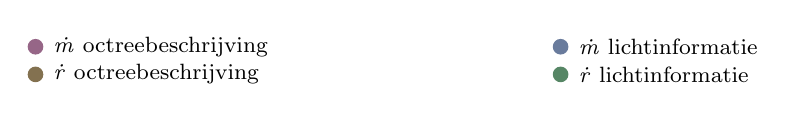
\begin{tikzpicture}
      \node (legend:1) at (0.1\textwidth,   0pt) [legend-point, fill={m-octree}, label=right:{\footnotesize $\mathit{\dot{m}}$ octreebeschrijving}] {};
      \node (legend:2) at (0.1\textwidth, -10pt) [legend-point, fill={r-octree}, label=right:{\footnotesize $\mathit{\dot{r}}$ octreebeschrijving}] {};
      
      \node (legend:3) at (0.65\textwidth,   0pt) [legend-point, fill={m-data},   label=right:{\footnotesize $\mathit{\dot{m}}$ lichtinformatie}] {};
      \node (legend:4) at (0.65\textwidth, -10pt) [legend-point, fill={r-data},   label=right:{\footnotesize $\mathit{\dot{r}}$ lichtinformatie}] {};
    \end{tikzpicture}
  \end{subfigure}\hfill\\
  \begin{adjustbox}{minipage=\textwidth, scale=0.55}
    \begin{subfigure}[b]{0.8\textwidth}
      \centering
      \def\svgwidth{\textwidth}
      \input{./img/raw/hs-seed-mem/seed_spaceship-indoor_70.pdf_tex}
      \caption{Spaceship Indoor: $70$ lichten.}
      \label{fig:hs-seed-memory::si-low}
    \end{subfigure}
  \end{adjustbox} %
  %
  \begin{adjustbox}{minipage=\textwidth, scale=0.55}
    \begin{subfigure}[b]{0.8\textwidth}
      \centering
      \def\svgwidth{\textwidth}
      \input{./img/raw/hs-seed-mem/seed_spaceship-indoor_1260.pdf_tex}
      \caption{Spaceship Indoor: $1260$ lichten.}
      \label{fig:hs-seed-memory::si-high}
    \end{subfigure}
  \end{adjustbox} \\
  %
  \begin{adjustbox}{minipage=\textwidth, scale=0.55}
    \begin{subfigure}[b]{0.8\textwidth}
      \centering
      \def\svgwidth{\textwidth}
      \input{./img/raw/hs-seed-mem/seed_pipers-alley_58.pdf_tex}
      \caption{Piper's Alley: $58$ lichten.}
      \label{fig:hs-seed-memory::pa-low}
    \end{subfigure}
  \end{adjustbox} %
  %
  \begin{adjustbox}{minipage=\textwidth, scale=0.55}
    \begin{subfigure}[b]{0.8\textwidth}
      \centering
      \def\svgwidth{\textwidth}
      \input{./img/raw/hs-seed-mem/seed_pipers-alley_1044.pdf_tex}
      \caption{Piper's Alley: $1044$ lichten.}
      \label{fig:hs-seed-memory::pa-high}
    \end{subfigure}
  \end{adjustbox} \\
  %
  \begin{adjustbox}{minipage=\textwidth, scale=0.55}
    \begin{subfigure}[b]{0.8\textwidth}
      \centering
      \def\svgwidth{\textwidth}
      \input{./img/raw/hs-seed-mem/seed_ziggurat-city_65.pdf_tex}
      \caption{Ziggurat City: $65$ lichten.}
      \label{fig:hs-seed-memory::zc-low}
    \end{subfigure}
  \end{adjustbox} %
  %
  \begin{adjustbox}{minipage=\textwidth, scale=0.55}
    \begin{subfigure}[b]{0.8\textwidth}
      \centering
      \def\svgwidth{\textwidth}
      \input{./img/raw/hs-seed-mem/seed_ziggurat-city_1170.pdf_tex}
      \caption{Ziggurat City: $1170$ lichten.}
      \label{fig:hs-seed-memory::zc-high}
    \end{subfigure}
  \end{adjustbox}
  \caption{Overzicht van het geheugengebruik van de verbindingloze octree
           bij verschillende seed-waardes.}
  \label{fig:hs-seed-memory}
\end{figure}

